\lecture{2}{03.09.2020}{Análise da Mobilidade}

Conceitos complementares:
\begin{description}
    \item[Elemento de par cinemático] é o que permite a um elo se conectar à outro
    \item[Elo "$i$-nário"] possui $i$ elementos de par cinemático
\end{description}

\begin{figure}[H]
    \centering
    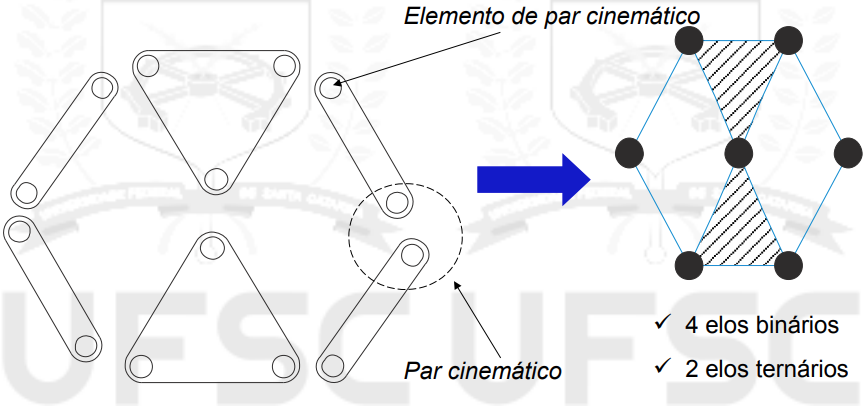
\includegraphics[width=0.8\textwidth]{figures/exemplo_elos_i_narios.png}
    \caption{Exemplo de elos $i$-nários.}
    \label{fig:figures-exemplo_elos_i_narios-png}
\end{figure}

\section*{Conectividade e Restrição}

\begin{definition}
    O número de graus de liberdade de movimento relativo entre dois corpos conectados é chamado \emph{Conectividade de juntas} e é denotado por $f_i$ para a $i$-ésima junta.

    A quantidade de graus de liberdade restringidos por um par cinemático é chamada \emph{Restrição} e é denotada por $c_i$ para a $i$-ésima junta.

    Estes dois conceitos se relacionam ao espaço de trabalho por \[
    c_i = \lambda - f_i
    \].
\end{definition}

Assim, pode-se derivar a equação que rege a quantidade de grau "líquido" de liberdade de uma cadeia.

\begin{definition}
    (Equação Geral da Mobilidade) A diferença entre as possibilidades de movimento dos elos móveis e as restrições de cada junta, é chamada Equação Geral da Mobilidade de uma cadeia e pode ser representada como \[
    M = \left( n-1 \right) \lambda - \sum_{i=1}^{j} c_i
\] ou \[
f_i = 1 \implies M = \left( n-1-j \right) \lambda + j
\], onde $n$ é o número de elos e $j$ é o número de juntas. Note que a mobilidade sempre é determinada a partir de um dos elos, por isso $(n-1)$ que é o número de corpos livres.
\end{definition}

\begin{note}
    Também é possível calcular a mobilidade através do número de circuitos \[
    v -1 = j - i
    \]. O número de circuitos também é utilizado como um \emph{índice de complexidade}.
\end{note}
